\documentclass[tikz]{standalone}
\usetikzlibrary{shapes,arrows.meta}
\begin{document}
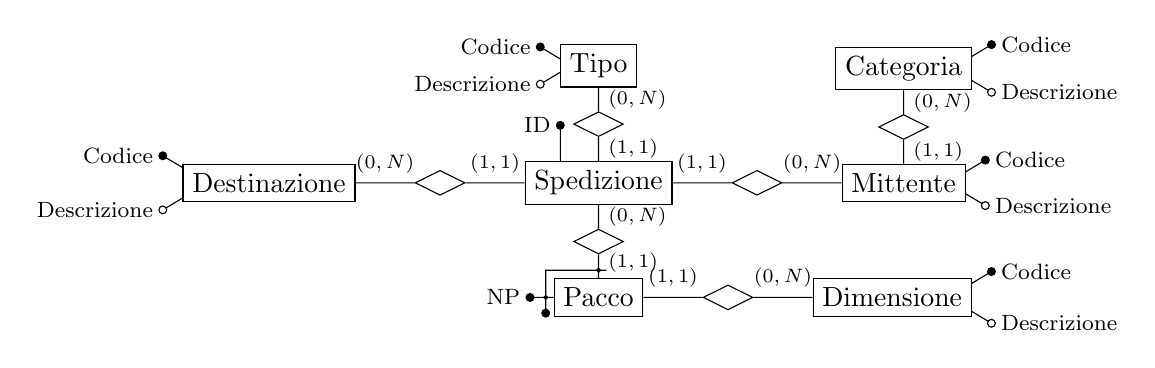
\begin{tikzpicture}
    \draw

    %%* Attributi:
    %%  node[draw, circle, inner sep=1pt, fill=black]{}node[right]{\footnotesize A}
    %%? Distanza orizzontale: E -(0.25,0.x)- A
    %%? Distanza verticale: E -(0,x * 0.22)- A

    %%* Cardinalità:
    %%  node[below right]{\scriptsize $(0,N)$}
    %%  node[above right]{\scriptsize $(0,N)$}
    %%  node[midway, above]{\scriptsize $(0,N)$}

    %%* Relazione:
    %%  node[draw, diamond, shape aspect=2, inner sep=3pt, anchor=90](r1){}
    %%  node[draw, diamond, shape aspect=2, inner sep=0.2pt, anchor=180](r2){R2}

    %%* Entità:
    %%  node[draw, rectangle, anchor=90](e1){}
    %%? Distanza verticale: E -(0.3)- R -(0.3) E
    %%? Distanza orizzontale: E -(0.75)- R -(0.75)- E

    %%* Destinazione
    (0,0)node[draw, rectangle, anchor=180](e1){Destinazione}
    (e1.0)--++(0.75,0)node[draw, diamond, shape aspect=2, inner sep=3pt, anchor=180](r1){}node[midway, above]{\scriptsize $(0,N)$}

    (e1.190)--++(-0.25,-0.15)node[draw, circle, inner sep=1pt, fill=white]{}node[left]{\footnotesize Descrizione}
    (e1.170)--++(-0.25,0.15) node[draw, circle, inner sep=1pt, fill=black]{}node[left]{\footnotesize Codice}


    %%* Spedizione
    (r1.0)--++(0.75,0)node[draw, rectangle, anchor=180](e2){Spedizione}node[midway, above]{\scriptsize $(1,1)$}
    (e2.90)--++(0,0.3)node[draw, diamond, shape aspect=2, inner sep=3pt, anchor=270](r2){}node[midway, right]{\scriptsize $(1,1)$}
    (e2.0)--++(0.75,0)node[draw, diamond, shape aspect=2, inner sep=3pt, anchor=180](r3){}node[midway, above]{\scriptsize $(1,1)$}
    (e2.270)--++(0,-0.3)node[draw, diamond, shape aspect=2, inner sep=3pt, anchor=90](r4){}node[midway, right]{\scriptsize $(0,N)$}
    
    (e2.150)--++(0,0.45)node[draw, circle, inner sep=1pt, fill=black]{}node[left]{\footnotesize ID}

    %%* Tipo
    (r2.90)--++(0,0.3)node[draw, rectangle, anchor=270](e3){Tipo}node[midway, right]{\scriptsize $(0,N)$}

    (e3.190)--++(-0.25,-0.15)node[draw, circle, inner sep=1pt, fill=white]{}node[left]{\footnotesize Descrizione}
    (e3.170)--++(-0.25,0.15) node[draw, circle, inner sep=1pt, fill=black]{}node[left]{\footnotesize Codice}


    %%* Mittente
    (r3.0)--++(0.75,0)node[draw, rectangle, anchor=180](e4){Mittente}node[midway, above]{\scriptsize $(0,N)$}
    (e4.90)--++(0,0.3)node[draw, diamond, shape aspect=2, inner sep=3pt, anchor=270](r5){}node[midway, right]{\scriptsize $(1,1)$}
    
    (e4.350)--++(0.25,-0.15)node[draw, circle, inner sep=1pt, fill=white]{}node[right]{\footnotesize Descrizione}
    (e4.10)--++(0.25,0.15) node[draw, circle, inner sep=1pt, fill=black]{}node[right]{\footnotesize Codice}


    %%* Categoria
    (r5.90)--++(0,0.3)node[draw, rectangle, anchor=270](e5){Categoria}node[midway, right]{\scriptsize $(0,N)$}

    (e5.350)--++(0.25,-0.15)node[draw, circle, inner sep=1pt, fill=white]{}node[right]{\footnotesize Descrizione}
    (e5.10)--++(0.25,0.15) node[draw, circle, inner sep=1pt, fill=black]{}node[right]{\footnotesize Codice}

    %%* Pacco
    (r4.270)--++(0,-0.2)node[draw, circle, inner sep=0.5pt, fill=black](a){}node[midway, right]{\scriptsize $(1,1)$}--++(0,-0.1)node[draw, rectangle, anchor=90](e6){Pacco}
    (e6.0)--++(0.75,0)node[draw, diamond, shape aspect=2, inner sep=3pt, anchor=180](r6){}node[midway, above]{\scriptsize $(1,1)$}

    (e6.180)--++(-0.1,0)node[draw, circle, inner sep=0.5pt, fill=black](b){}--++(-0.2,0)node[draw, circle, inner sep=1pt, fill=black]{}node[left]{\footnotesize NP}

    (a)++(0.1,0)-|(b)--++(0,-0.2)node[draw, circle, inner sep=1pt, fill=black]{}


    %%* Dimensione
    (r6.0)--++(0.75,0)node[draw, rectangle, anchor=180](e7){Dimensione}node[midway, above]{\scriptsize $(0,N)$}

    (e7.350)--++(0.25,-0.15)node[draw, circle, inner sep=1pt, fill=white]{}node[right]{\footnotesize Descrizione}
    (e7.10)--++(0.25,0.15) node[draw, circle, inner sep=1pt, fill=black]{}node[right]{\footnotesize Codice}
    
    ;
\end{tikzpicture}
\end{document}